\chapter{Implementacija i korisničko sučelje}
		
		
		\section{Korištene tehnologije i alati}
		
			
			Komunikacija u timu realizirana je korištenjem platforme \underline{Microsoft Teams}\footnote{\url{https://www.microsoft.com/hr-hr/microsoft-365/microsoft-teams/}}. 
			Za izradu UML dijagrama korišten je alat \underline{Astah Professional}\footnote{\url{https://astah.net/products/astah-professional/}}, a kao sustav za upravljanje izvornim kodom \underline{Git}\footnote{\url{https://git-scm.com/}}. 
			Udaljeni repozitorij projekta je dostupan na web platformi \underline{GitLab}\footnote{\url{https://gitlab.com/}}.
			\par
			Kao razvojno okruženje korišten je \underline{IntelliJ IDEA}\footnote{\url{https://www.jetbrains.com/idea/}} - integrirano razvojno okruženje (IDE) tvrtke JetBrains. 
			Prvenstveno se koristi za razvoj računalnih programa za operacijski sustav Windows, kao i za web-stranice, web-aplikacije, web-usluge i mobilne aplikacije.
			\par
			Za razvoj korisničkog sučelja i frontenda korišten je uređivač teksta \underline{VSCode}\footnote{\url{https://code.visualstudio.com/}}. Taj uređivač teksta je danas jedan od najrasprostranjenijih i koristi se u svim sferama industrije. 
            \par
            Aplikacija je napisana u \underline{Javi}\footnote{\url{https://www.java.com/en/}} koristeći ekosustav \underline{Java Spring}\footnote{\url{https://spring.io/}} za
            izradu backenda te \underline{AngularJS}\footnote{\url{https://angularjs.org/}} i jezik \underline{JavaScript}\footnote{\url{https://www.javascript.com/}} za izradu frontenda. 
            \par
            Baza podataka (\underline{PostgreSQL}\footnote{\url{https://www.postgresql.org/}}) se nalazi na poslužitelju u oblaku \underline{Digital Ocean}\footnote{\url{https://www.digitalocean.com/}}.

            
            \vspace*{\fill}

			
			\eject
		
	
		\section{Ispitivanje programskog rješenja}
		Nakon što smo završili s izradom testirali smo rad aplikacije koristeći JUnit tehnologiju i Selenium WebDriver. Testovi su većinom dali zadovoljavajuće rezultate te možemo zaključiti da smo uspjeli implementirati zadane funkcionalnosti.
		
		
		\subsection{Ispitivanje komponenti}
		Za ispitivanje komponenti koristili smo JUnit tehnologiju. JUnit okvir je za testiranje komponenti sustava programiranog u Javi. Za simuliranje dohvaćanja podataka iz baze koristili smo okvir Mockito. Ispitali smo funkcionalnosti ažuriranja profila, ažuriranja zadatka i dodavanja novog zadatka. Koriste se objekti tipa EmployeeController i TasksController nad kojima se pozivaju ispitivane funkcionalnosti te objekti tipa EmployeeRepository, TaskRepository i TeamRepository koji su potrebni za dohvaćanje podataka korištenih u funkcijama.
		\newline
		\newline
		\textbf{Ažuriranje profila}
		
		Pozivom funkcije updateEmployeeWithUsername iz klase EmployeeController želimo zaposleniku uspješno promijeniti prezime. Na kraju uspoređujemo je li prezime ažuriranog zaposlenika jednako željenom novom prezimenu.
		\begin{verbatim}
			
			@Test
			public void editProfileCorrectly() {
				  
				  Employee employee = new   Employee("iva123","Iva","Ivić","0910000000",
				  "iva@fer.hr",ClearanceLevel.DEVELOPER,null,null);
				
				  Mockito.when(employeeRepository.findByUsername(
				  employee.getUsername())).thenReturn(Optional.of(employee));
				
				  String newSurname="Ivančić";
				  Employee employeeWithNewSurname = new Employee(employee.getUsername(),
				  employee.getName(),newSurname,employee.getPhoneNumber(), employee.getEmail(),
				  employee.getClearanceLevel(),employee.getTeam(),employee.getTasks());
				
				  String[] expected = {newSurname};
				  String[] result = {employeeController.updateEmployeeWithUsername(
					  employee.getUsername(),employeeWithNewSurname).getBody().getSurname()};
				  Assertions.assertArrayEquals(expected,result);
			}
			
		\end{verbatim}
		U idućem testu pozivom iste funkcije želimo neuspješno ažurirati korisnika pokušajem mijenjanja korisničkog imena, koje se se bi smjelo mijenjati. Na kraju uspoređujemo je li dobivena statusna poruka jednaka očekivanoj "404 NOT\textunderscore FOUND" što bi značilo da aplikacija na pobuđenu situaciju prikladno odgovara.
		
		\begin{verbatim}
			
			@Test
			public void editProfileIncorrectly() {
				  
				  Employee employee = new Employee("iva123","Iva","Ivić","0910000000",
				  "iva@fer.hr",ClearanceLevel.DEVELOPER,null,null);
				
				  String newUsername="iva1234";
				  Employee employeeWithNewUsername = new Employee(newUsername,
				  employee.getName(),employee.getSurname(),employee.getPhoneNumber(),
				  employee.getEmail(),employee.getClearanceLevel(),
				  employee.getTeam(),employee.getTasks());
				
				  String[] expected = {"404 NOT_FOUND"};
				  String[] result = {employeeController.updateEmployeeWithUsername(
					  employee.getUsername(),employeeWithNewUsername).getStatusCode().toString()};
				  Assertions.assertArrayEquals(expected,result);
			}
			
		\end{verbatim}
		\textbf{Ažuriranje zadatka}
		
		Pozivom funkcije updateTask iz klase TasksController želimo zadatku uspješno promijeniti prioritet. Na kraju uspoređujemo je li prioritet ažuriranog zadatka jednak željenom novom prioritetu.
		\begin{verbatim}
			
			@Test
			public void editTaskCorrectly(){
				  
				  Employee coordinator = new Employee("iva123","Iva","Ivić","0910000000",
				  "iva@fer.hr",ClearanceLevel.COORDINATOR,null,null);
				  WorkGroup workGroup = new WorkGroup(coordinator,null);
				  Team team = new Team(null,workGroup,null);
				  team.setTeamId(Long.valueOf(101));
				  Task task = new Task("Testiranje sustava","Potrebno testirati sustav.",
				  TaskPriority.HIGH,new Date(2020,1,2),TaskStatus.BACKLOG,null);
				  task.id = Long.valueOf(22);
				
				  Mockito.when(taskRepository.findById(
				  task.getId())).thenReturn(Optional.of(task));
				
				  TaskPriority newPriority = TaskPriority.VERY_HIGH;
				  Task taskWithNewPriority = new Task(task.getName(), task.getDescription(),
				  newPriority,task.getDeadline(),task.getStatus(),task.getEmployee());
				  taskWithNewPriority.id = task.getId();
				
				  TaskPriority[] expected = {newPriority};
				  TaskPriority[] result = {tasksController.updateTask(task.getId(),
					taskWithNewPriority).getBody().getPriority()};
				  Assertions.assertArrayEquals(expected,result);
			}
			
		\end{verbatim}
		Pozivom iste funkcije želimo neuspješno ažurirati zadatak pokušajem postavljanja praznog naziva zadatka, što ne bi smjelo prolaziti. Uspoređujemo je li dobivena statusna poruka jednaka očekivanoj "400 BAD\textunderscore REQUEST" što bi značilo da aplikacija dobro reagira na naš loš zahtjev.
		
		\begin{verbatim}
			
			@Test
			public void editTaskIncorrectly(){
				  
				  Team team = new Team(null,null,null);
				  team.setTeamId(Long.valueOf(101));
				  Task task = new Task("Testiranje sustava","Potrebno testirati sustav.",
				  TaskPriority.HIGH,new Date(2020,1,2),TaskStatus.BACKLOG,null);
				  task.id = Long.valueOf(22);
				
				  Mockito.when(taskRepository.findById(
				  task.getId())).thenReturn(Optional.of(task));
				
				  Task taskWithNoName = new Task(null, task.getDescription(),
				  task.getPriority(),task.getDeadline(),task.getStatus(),task.getEmployee());
				  taskWithNoName.id = task.getId();
				
				  String[] expected = {"400 BAD_REQUEST"};
				  String[] result = {tasksController.updateTask(task.getId(),
					  taskWithNoName).getStatusCode().toString()};
				  Assertions.assertArrayEquals(expected,result);
			}
			
		\end{verbatim}
		\textbf{Dodavanje zadatka}
		
		Funkcijom createTask iz klase TasksController želimo uspješno dodati zadatak. Na kraju uspoređujemo jesu li atributi stvorenog zadatka jednaki željenim.
		\begin{verbatim}
			
			@Test
			public void addTaskCorrectly(){
				  
				  Team team = new Team(null,null,null);
				  team.setTeamId(Long.valueOf(101));
				  Mockito.when(teamRepository.findById(
				  team.getTeamId())).thenReturn(Optional.of(team));
				
				  Task task = new Task("Testiranje sustava","Potrebno testirati sustav.",
				  TaskPriority.HIGH,new Date(2020,1,2),TaskStatus.BACKLOG,null);
				  Mockito.when(taskRepository.save(any(Task.class))).thenReturn(task);
				  Task createdTask = tasksController.createTask(team.getTeamId(),task).getBody();
				
				  String[] expected = {task.getName(),task.getDescription(),
					  task.getPriority().toString(),task.getDeadline().toString()};
				  String[] result = {createdTask.getName(),createdTask.getDescription(),
					  createdTask.getPriority().toString(),createdTask.getDeadline().toString()};
				  Assertions.assertArrayEquals(expected,result);
			}
			
		\end{verbatim}
		Pozivom iste funkcije želimo neuspješno dodati bezimeni zadatak. Na kraju uspoređujemo je li stvoreni zadatak jednak null vrijednosti što bi značilo da aplikacija odbija stvoriti takav zadatak.
		
		\begin{verbatim}
			
			@Test
			public void addTaskIncorrectly(){
				  
				  Team team = new Team(null,null,null);
				  team.setTeamId(Long.valueOf(101));
				  Mockito.when(teamRepository.findById(
				  team.getTeamId())).thenReturn(Optional.empty());
				
				  Task taskWithoutName = new Task(null,"Potrebno testirati sustav.",
				  TaskPriority.HIGH,new    Date(2020,1,2),TaskStatus.BACKLOG,null);
				
				  Task[] expected = {null};
				  Task[] result = {tasksController.createTask(team.getTeamId(),
					  taskWithoutName).getBody()};
				  Assertions.assertArrayEquals(expected,result);
			}
			
		\end{verbatim}
		\begin{figure}[H] 
			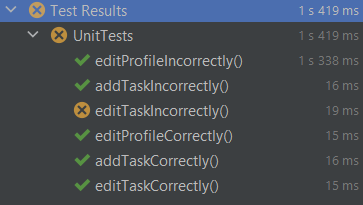
\includegraphics[width=\textwidth]{slike/unitTestRezultati.png}
			\caption{Rezultati ispitivanja komponenti}
		\end{figure}
		
		
		
		
		
		
		
		
		
		
		\subsection{Ispitivanje sustava}
		
		Sustav smo ispitivali pomoću Selenium WebDriver okvira. Selenium WebDriver omogućuje ispitivanje sustava za koji je potrebna interakcija s internetskim preglednikom. Koristili smo Google Chrome preglednik. Ispitali smo funkcionalnosti uređivanja profila, uređivanja zadatka i dodavanja zadatka. Koriste se pomoćna metoda void login(WebDriver driver, String username, String password) za prijavu željenog korisnika u sustav i void logout(WebDriver driver) za odjavu korisnika. U main metodi definirane su potrebne vrijednosti za poziv svake funkcije.
		
		\textbf{Ažuriranje profila}
		
		Cilj prvog testa uspješno je ažuriranje korisnika. Funkcija editProfileCorrectly prvo prijavljuje željenog korisnika (korisničkog imena mhren), pritiskom na gumb otvara profil, odabire opciju za uređivanje, mijenja broj mobitela i mail te sprema promijenjene podatke. Test je uspješan ukoliko su broj mobitela i mail korisničkog profila postali jednaki željenima.
		\begin{verbatim}
			
			public static String editProfileCorrectly(WebDriver driver,String username,
			String password,String newPhone,String newMail) {
				
				  login(driver,username,password);
				
				  driver.findElement(By.id("openProfile")).click();
				  driver.findElement(By.id("editProfile")).click();
				
				  WebElement element = driver.findElement(By.id("brMob"));
				  element.clear();
				  element.sendKeys(newPhone);
				
				  element = driver.findElement(By.id("eMail"));
				  element.clear();
				  element.sendKeys(newMail);
				
				  driver.findElement(By.id("spremi")).click();
				  boolean success=driver.findElement(By.id("mail")).getText().equals(newMail)&&
				  driver.findElement(By.id("mob")).getText().equals(newPhone);
				
				  return "editProfileCorrectly success: " + success;
			}
			
		\end{verbatim}
		Cilj drugog testa neuspješno je ažuriranje korisnika. Na početku funkcije editProfileIncorrectly već smo prijavljeni u sustav. Ponovno otvaramo profil i želimo ga urediti, ovaj 
		put pokušavamo postaviti prazno korisničko ime, što se ne bi smjelo prihvatiti. Uspjehom smatramo ako u određenom vremenu iskoči prozor s upozorenjem koji označava da se podatci nisu promijenili. Ako se prozor pojavi na njemu pritišćemo "U redu". Odjavljujemo trenutnog korisnika zato što nam za idući test treba drugi korisnik.
		\begin{verbatim}
			
			public static String editProfileInorrectly(WebDriver driver){
				  
				  driver.findElement(By.id("editProfile")).click();
				  WebElement element = driver.findElement(By.id("korIme"));
				  element.clear();
				  element.sendKeys(null);
				  driver.findElement(By.id("spremi")).click();
				
				  boolean success;
				
				  try {
					    WebDriverWait wait = new WebDriverWait(driver, 2);
					    wait.until(ExpectedConditions.alertIsPresent());
					    driver.switchTo().alert().accept();
					    success = true;
				  }catch(TimeoutException ex){
					    success = false;
				  }
				
				  driver.findElement(By.id("zatvori")).click();
				  logout(driver);
				  return "editProfileIncorrectly success: " + success;
			}
			
		\end{verbatim}
		\textbf{Dodavanje zadatka}
		
		Želimo uspješno dodati zadatak. U fuknciji addTaskCorrectly prvo se prijavljujemo s korisničkim podatcima koordinatora, pritišćemo gumb za dodavanje zadatka, dajemo mu ime, opis, prioritet i rok te ga spremamo. Uspješni smo ukoliko je broj zadataka na kanban ploči za jedan viši od broja zadataka na ploči prije pokušaja dodavanja zadatka.
		\begin{verbatim}
			
			public static String addTaskCorrectly(WebDriver driver,String username, 
			String password,String taskName,String description,
			TaskPriority priority,String deadline){
				
				  login(driver,username,password);
				
				  int numberOfTasks = driver.findElements(By.id("task")).size();
				  driver.findElement(By.id("addTask")).click();
				
				  driver.findElement(By.id("taskName")).sendKeys(taskName);
				  driver.findElement(By.id("description")).sendKeys(description);
				  driver.findElement(By.id("priority")).sendKeys(priority.toString());
				  driver.findElement(By.id("deadline")).sendKeys(deadline);
				  driver.findElement(By.id("add")).click();
				
				  boolean success=driver.findElements(By.id("task")).size()==numberOfTasks+1;
				  return "addTaskCorrectly success: " + success;
			}
			
		\end{verbatim}
		Želimo neuspješno dodati zadatak. U funkciji addTaskIncorrectly pritišćemo gumb za dodavanje zadatka, upisujemo naziv, opis te prioritet i rok neispravnih oblika. Spremamo podatke. Uspjehom smatramo ako u određenom vremenu iskoči prozor upozorenja koji označuje da zadatak nije dodan. Ako se prozor pojavi na njemu pritišćemo "U redu".
		
		\begin{verbatim}
			
			public static String addTaskIncorrectly(WebDriver driver,String taskName,
			String description){
				
				  driver.findElement(By.id("addTask")).click();
				
				  driver.findElement(By.id("taskName")).sendKeys(taskName);
				  driver.findElement(By.id("description")).sendKeys(description);
				  driver.findElement(By.id("priority")).sendKeys("unknown");
				  driver.findElement(By.id("deadline")).sendKeys("unknown");
				  driver.findElement(By.id("add")).click();
				
				  boolean success;
				
				  try {
					    WebDriverWait wait = new WebDriverWait(driver, 2);
					    wait.until(ExpectedConditions.alertIsPresent());
					    driver.switchTo().alert().accept();
					    success = true;
				  }catch(TimeoutException ex){
					    success = false;
				  }
				  return "addTaskIncorrectly success: " + success;
			}
			
		\end{verbatim}
		\textbf{Ažuriranje zadatka}
		
		Cilj ovog testa uspješno je uređivanje zadatka. Prije poziva funkcije editTaskCorrectly nalazimo se na kanban ploči iz prethodnog testa. Pronalazimo jedan gumb za uređivanje zadatka koji možemo pritisnuti (tj. jedan zadatak koji smo ranije preuzeli te ga imamo pravo urediti). Pritišćemo pronađeni gumb, zadatku mijenjamo opis i spremamo promjene. Uspjehom smatramo ako se nakon određenog vremena nije pojavio skočni prozor s upozorenjem koji bi signalizirao da zadatak nije uspješno promijenjen.
		\begin{verbatim}
			
			public static String editTaskCorrectly(WebDriver driver, String description){
				  
				  ArrayList<WebElement> editButtons=(ArrayList<WebElement>)driver.findElements(
				  By.id("editTask"));
				  for(WebElement editButton:editButtons){
					    if(editButton.isEnabled()){
						      editButton.click();
						      break;
					    }
				  }
				
				  WebElement element = driver.findElement(By.id("description"));
				  element.clear();
				  element.sendKeys(description);
				
				  driver.findElement(By.id("saveTask")).click();
				
				  boolean success;
				  try {
					    WebDriverWait wait = new WebDriverWait(driver, 2);
					    wait.until(ExpectedConditions.alertIsPresent());
					    driver.switchTo().alert().accept();
					    success = false;
				  }catch(TimeoutException ex){
					    success = true;
				  }
				  return "editTaskCorrectly success: " + success;
			}
			
		\end{verbatim}
		Posljednjim testom želimo neuspješno ažurirati zadatak. U funkciji editTaskIncorrectly pritišćemo gumb za uređivanje zadatka, postavljamo prazni prioritet i spremamo promjene. Uspjehom smatramo ako se nakon nekog vremena pojavi skočni prozor koji označava da je nešto pošlo po krivu.
		
		\begin{verbatim}
			
			public static String editTaskIncorrectly(WebDriver driver){
				  
				  ArrayList<WebElement> editButtons=
				  (ArrayList<WebElement>)driver.findElements(By.id("editTask"));
				  for(WebElement editButton:editButtons){
					    if(editButton.isEnabled()){
						      editButton.click();
						      break;
					    }
				  }
				
				  WebElement element = driver.findElement(By.id("priority"));
				  element.clear();
				
				  driver.findElement(By.id("saveTask")).click();
				
				  boolean success;
				  try {
					    WebDriverWait wait = new WebDriverWait(driver, 2);
					    wait.until(ExpectedConditions.alertIsPresent());
					    driver.switchTo().alert().accept();
					  success = true;
				  }catch(TimeoutException ex){
					    success = false;
				  }
				  return "editTaskInorrectly success: " + success;
			}
			
			
		\end{verbatim}
		
		\begin{figure}[H] 
			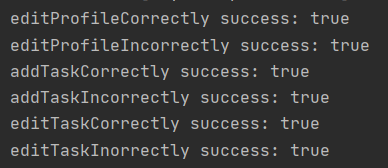
\includegraphics[width=\textwidth]{slike/systemTestRezultati.png}
			\caption{Rezultati ispitivanja sustava}
		\end{figure}
			
			\eject 
		
		
		\section{Dijagram razmještaja}
			
			Dijagrami razmještaja prikazuju topologiju sustava i odnos sklopovskih i programskih dijelova. Olakšavaju nam vizualizaciju razmještaja fizičkog dijela sustava i sklopovlja. Sustav se sastoji od korisničkog i poslužiteljskog računala. Korisnik na svojem računalu preko web preglednika pristupa aplikaciji. Korisničko računalo komunicira s poslužiteljskim računalom preko HTTP veze. Na poslužiteljskom se računalu nalaze HTTP poslužitelj, REST poslužitelj i poslužitelj baze podataka. 
			
			\begin{figure}[H]
				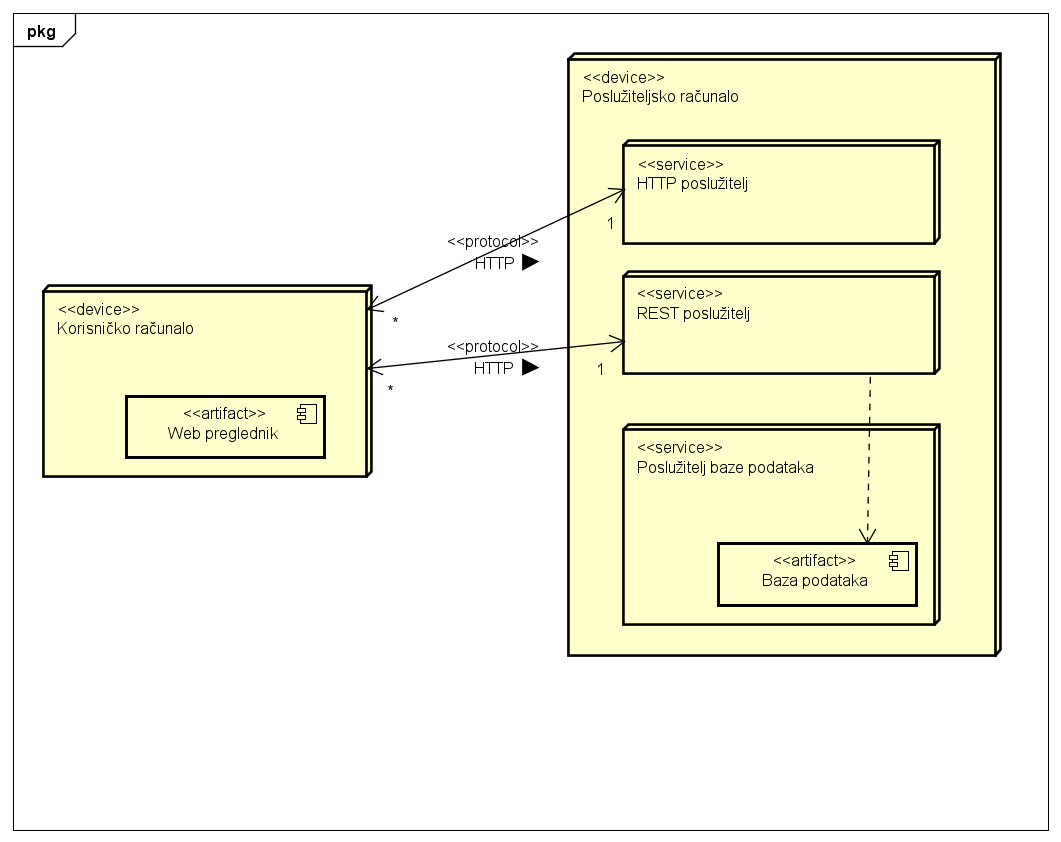
\includegraphics[width=\textwidth]{slike/dijagram_razmjestaja.png}
				\centering
				\caption{Dijagram razmještaja}
				\label{fig:dijagram_razmjestaja}
			\end{figure}
			
			\eject 
		
		\section{Upute za puštanje u pogon}
		
		\subsection{Operacijski sustav}
		Pretpostavlja se operacijski sustav iz Linux obitelji, na primjer \underline{Ubuntu 20.04}\footnote{\url{https://ubuntu.com/}}.
		
		\subsection{Preuzimanje programskog rješenja}
		Potrebno je instalirati paket \texttt{git} naredbom \textbf{sudo apt install git}. Zatim je potrebno pokrenuti naredbu \textbf{git clone \url{https://gitlab.com/henri_ohm/worldpiis.git}} kako bi se preuzelo programsko rješenje. Ovom naredbom će se stvoriti direktorij \texttt{worldpiis} (dalje \$PROJECT\_ROOT) koji sadrži sve potrebne datoteke za pokretanje aplikacije.
		
		\subsection{Baza podataka}
		Potrebnu je preuzeti i instalirati najnoviju verziju paketa PostgreSQL. Pokretanjem naredbe \textbf{sudo apt install postgresql-12} potreban paket se preuzima i instalira, te se stvaraju daemon servisi koji pokreću bazu podataka prilikom pokretanja računala.
		
		\subsection{Konfiguracija poslužitelja baze podataka}
		Ovako instalirana baza podataka sluša zahtjeve sa adrese 127.0.0.1 na vratima 5432. Ovakva konfiguracija dovoljna je za potrebe ovog projekta. Također je potrebno osigurati da u bazi postoji \textbf{korisnik `postgres`} sa \textbf{lozinkom `postgres`}. Potrebno je osigurati i da na računalu postoji korisnik `postgres`, no to bi sama instalacija paketa već trebala osigurati.
		
		\subsection{Konfiguracija baze podataka}
		Sve potrebne tablice, ograničenja i veze će inicijalizirati REST poslužitelj kad se pokrene, pa je potrebno osigurati samo prije navedene uvjete kako bi baza radila.
		
		\subsection{Punjenje baze podataka}
		Za punjenje baze podataka dostupna je skripta na lokaciji \textbf{\$PROJECT\_ROOT/db/fill.sql}. Ova skripta može se pokrenuti tako da se prvo pokrene sučelje s bazom, naredbom \textbf{sudo -i -u postgres psql}, a zatim se pokrene naredba \textbf{\textbackslash i db/fill.sql}. Ovdje se pretpostavlja da je korisnik postavljen u korijenskom direktoriju projekta.
		
		\subsection{Pokretanje baze podataka}
		Baza podataka pokreće se kada se računalo upali, no ukoliko postoje problemi, može se pokrenuti naredba \textbf{sudo systemctl enable postgresql}, koja će omogućiti pokretanje baze prilikom pokretanja računala, te naredba \textbf{sudo systemctl start postgresql} koja će pokrenuti bazu podataka jednom. Prva naredba osigurava pokretanje baze prilikom pokretanja računala.
		
		\subsection{Javna vrata servera}
		Potrebno je osigurati da su vrata 80 i vrata 8080 otvorena javnosti, što je moguće naredbom \textbf{sudo ufw allow 80} i \textbf{sudo ufw allow 8080}. Ovaj postupak omogućuje poslužitelju primanje zahtjeva na ta dva vrata. Vrata 80 su dobro poznata vrata za posluživanje HTTP zahtjeva, a na vrata 8080 dolaziti će zahtjevi na REST poslužitelj.
		
		\subsection{Pokretanje web poslužitelja}
		Prije svega, potrebno je osigurati prisutnost Python interpretatora, što je moguće naredbom \textbf{sudo apt install python3}. Nadalje, da bi se web poslužitelj pokrenuo, potrebno je pozicionirati se u direktorij \textbf{\$PROJECT\_ROOT/web} i pokrenuti naredbu \textbf{sudo python3 -m http.server 80}. Prije toga, potrebno je osigurati da su vrata 80 slobodna, odnosno da nijedan drugi proces ne sluša na tim vratima.
		
		\subsection{Konfiguracija veze s bazom podataka}
		U datoteci \textbf{\$PROJECT\_ROOT/src/main/resources/application.properties} postavljene su iduće konfiguracijske varijable:
		\begin{itemize}
			\item \texttt{spring.datasource.url = jdbc:postgresql://localhost:5432/postgres}
			\item \texttt{spring.datasource.username = postgres}
			\item \texttt{spring.datasource.password = postgres}
		\end{itemize}
		Prva varijabla govori poslužitelju na koji URI treba slati zahtjeve bazi podataka. Druga i treća varijabla govore s kojim korisničkim imenom i lozinkom se ti zahtjevi trebaju slati.
		
		\subsection{Pokretanje REST poslužitelja}
		Prije nego što se pokrene REST poslužitelj, potrebno je osigurati prisutnost Jave 13 i programskog paketa Apache Maven. U tu svrhu, potrebno je pokrenuti naredbu \textbf{sudo apt install openjdk-13 maven}, koja će instalirati oba paketa u jednom potezu. Nakon toga, potrebno je pozicionirati se u korijenski direktorij i pokrenuti naredbu \textbf{mvn -N io.takari:maven:wrapper}, koja će instalirati potreban paket za pokretanje Spring aplikacije. Konačno, u korijenskom direktoriju potrebno je pokrenuti poslužitelj naredbom \textbf{./mvnw spring-boot:run}. Ukoliko su potrebne debugging poruke, moguće je staviti zastavice \underline{-e -X}.  
		
		\subsection{Konfiguriranje adrese spajanja}
		Na početku datoteke \textbf{\$PROJECT\_ROOT/web/app.js} dostupna je varijabla \textbf{REST\_base} koja govori na koju adresu i vrata frontend treba slati zahtjeve da bi dobio REST odgovore. Ova varijabla po potrebi se može mijenjati za lokalno testiranje ili kada se mijenja domena ili adresa aplikacije. 
		
		\subsection{Domena aplikacije}
		Kako bi aplikaciji bilo lakše pristupati, potrebno je registrirati domenu na bilokojem pružatelju domenskih imena. Za potrebe ovog projekta, korišten je \textbf{DuckDNS}\footnote{\url{https://www.duckdns.org/}}.
		
		\subsection{Korištenje aplikacije}
		Nakon svih ovih koraka, aplikacija je upogonjena i dostupna na registriranoj domeni. Aplikacija ovog projekta dostupna je na domeni \textbf{\url{worldpiis.duckdns.org}}.
		\eject 